% \iffalse
\documentclass[journal,12pt,twocolumn]{IEEEtran}
\usepackage{cite}
\usepackage{amsmath,amssymb,amsfonts,amsthm}
\usepackage{algorithmic}
\usepackage{graphicx}
\usepackage{textcomp}
\usepackage{xcolor}
\usepackage{txfonts}
\usepackage{listings}
\usepackage{enumitem}
\usepackage{mathtools}
\usepackage{gensymb}
\usepackage{comment}
\usepackage[breaklinks=true]{hyperref}
\usepackage{tkz-euclide}
\usepackage{listings}
\usepackage{gvv}
\def\inputGnumericTable{}
\usepackage[latin1]{inputenc}
\usepackage{color}
\usepackage{array}
\usepackage{longtable}
\usepackage{calc}
\usepackage{multirow}
\usepackage{hhline}
\usepackage{ifthen}
\usepackage{lscape}
\usepackage{caption}

\newtheorem{theorem}{Theorem}[section]
\newtheorem{problem}{Problem}
\newtheorem{proposition}{Proposition}[section]
\newtheorem{lemma}{Lemma}[section]
\newtheorem{corollary}[theorem]{Corollary}
\newtheorem{example}{Example}[section]
\newtheorem{definition}[problem]{Definition}
\newcommand{\BEQA}{\begin{eqnarray}}
\newcommand{\EEQA}{\end{eqnarray}}
\newcommand{\define}{\stackrel{\triangle}{=}}
\theoremstyle{remark}
\newtheorem{rem}{Remark}
\begin{document}

\bibliographystyle{IEEEtran}
\vspace{3cm}

\title{NCERT 11.9.4 8Q}
\author{EE22BTECH11010 - Venkatesh D Bandawar $^{*}$% <-this % stops a space
}
\maketitle
% \newpage
\bigskip

\renewcommand{\thefigure}{\theenumi}
\renewcommand{\thetable}{\theenumi}

\textbf{Question:} Find the sum to n+1 terms of series , whose $(n+1)^{th}$ term is : $(n+1)(n+2)(n+5)$.

\textbf{Solution}
\begin{table}[!h] 
\centering
\begin{tabular}{|c|c|c|}
\hline
    Parameter & Description & Value\\
    \hline
    $P(s)$ & Plant Transfer Function & $\frac{0.001}{s\brak{\frac{s}{0.5}+1}\brak{\frac{s}{100}+1}}$\\
    \hline
    $C(s)$ & Lag Compensator  & $\frac{100\brak{\frac{s}{10}+1}}{\frac{s}{0.1}+1}$\\
    \hline
    $T(s)$ & Loop gain  & $P(s) C(s)$ \\
    \hline
    $\omega$ & Angular Frequency & 3rad/s \\
    \hline
\end{tabular}

\caption{Given parameters}
\label{given parameters list}
\end{table}

from equation \eqref{eq:11.9.5.26.2} to \eqref{eq:11.9.5.26.4},\\
    \begin{align}
        X(z) &= \frac{z^{-1}\brak{1+4z^{-1}+z^{-2}}}{\brak{1-z^{-1}}^4} + \frac{8z^{-1}\brak{z^{-1}+1}}{\brak{1-z^{-1}}^3} \nonumber\\
        &+ \frac{17z^{-1}}{\brak{1-z^{-1}}^2}  + \frac{10}{1-z^{-1}}\\
        Y(z) &= X(z)U(z)\\
        &= \frac{z^{-1}\brak{1+4z^{-1}+z^{-2}}}{\brak{1-z^{-1}}^5} + \frac{8z^{-1}\brak{z^{-1}+1}}{\brak{1-z^{-1}}^4} \nonumber\\
        &+ \frac{17z^{-1}}{\brak{1-z^{-1}}^3} +\frac{10}{(1-z^{-1})^2}
    \end{align}
Using contour integration for inverse Z transformation,
    \begin{align}
        y(n) &= \frac{1}{2\pi j}\oint_c Y(z) z^{n-1} dz \\
        &= \frac{1}{2\pi j}\oint_c \frac{\brak{z^2+4z+1}}{\brak{z-1}^5} z^{n+1} dz  \nonumber\\
        &+ \frac{1}{2\pi j}\oint_c \frac{8\brak{z+1}}{\brak{z-1}^4} z^{n+1} dz   \nonumber\\
        &+ \frac{1}{2\pi j}\oint_c \frac{17}{\brak{z-1}^3} z^{n+1} dz + \frac{1}{2\pi j}\oint_c \frac{10}{(z-1)^2}z^{n+1} dz\\
        \because R&=\frac{1}{\brak {m-1}!}\lim\limits_{z\to a}\frac{d^{m-1}}{dz^{m-1}}\brak {{(z-a)}^{m}f\brak z}
    \end{align}
    \begin{align}
        R_1 &=\frac{1}{4!}\lim\limits_{z\to 1}\frac{d^4}{dz^4}\brak {(z-1)^5 \frac{\brak{z^2+4z+1}z^{n+1}}{\brak{z-1}^5}}\\
        &= \frac{(n+3)(n+2)(n+1)(n)}{4!} \nonumber\\
        & + \frac{4(n+2)(n+1)(n)(n-1)}{4!} \nonumber\\
        & + \frac{(n+1)(n)(n-1)(n-2)}{4!}\\
        R_2 &=\frac{1}{3!}\lim\limits_{z\to 1}\frac{d^3}{dz^3} \brak{(z-1)^4 \frac{8\brak{z+1}z^{n+1}}{\brak{z-1}^4}}\\
        &= \frac{8(n+2)(n+1)(n)}{3!} + \frac{8(n+1)(n)(n-1)}{3!}\\
        R_3 &=\frac{1}{2!}\lim\limits_{z\to 1}\frac{d^2}{dz^2} \brak{(z-1)^3 \frac{17z^{n+1}}{\brak{z-1}^3}}\\
        &= \frac{17(n+1)(n)}{2!}\\
        R_4 &=\frac{1}{1!}\lim\limits_{z\to 1} \frac{d}{dz} \brak{(z-1)^2\frac{10z^{n+1}}{(z-1)^2}}\\
        &= 10(n+1)\\
        \implies y(n1) &= R_1 + R_2 + R_3 + R_4\\
        &= \frac{n^2(n+1)^2}{4} + \frac{8(n)(n+1)(2n+1)}{6} \nonumber\\
        &+ \frac{17n(n+1)}{2} + 10(n+1)
    \end{align}

    \begin{figure}[!h] 
    \centering
    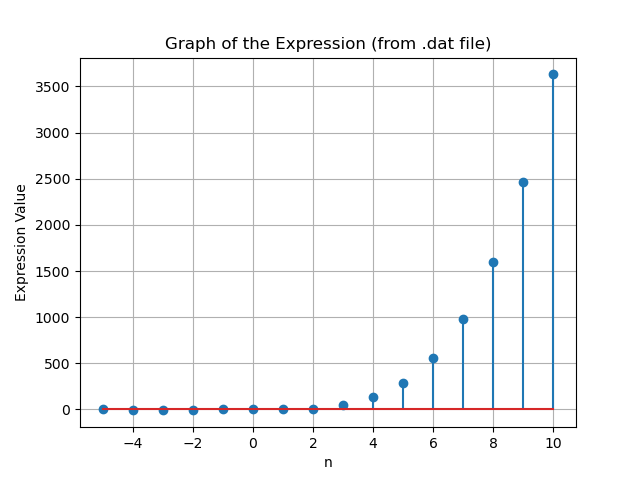
\includegraphics[width=\columnwidth]{figs/sumplot.png}
    \caption{$y(n)= \frac{n^2(n+1)^2}{4} + \frac{8(n)(n+1)(2n+1)}{6} + \frac{17n(n+1)}{2} + 10(n+1)$}
    \label{fig:Graph1_math.11.9.4.8}
    \end{figure}

\end{document}
